\documentclass[aps,prb,10pt,amsmath,amssymb,superscriptaddress]{revtex4-2}
\usepackage{hyperref}
\usepackage{graphicx,tikz}
\usepackage{mathtools}
\usepackage{array}
\usepackage{multirow}
\usepackage{orcidlink}
\usepackage{bm}
\usepackage{subfigure}

\def\be#1\ee{\begin{align}#1\end{align}}
\newcommand{\rmd}{\mathrm{d}}

\begin{document}
\title{Modifications}

\author{Hiroki Yoshida}
\date{\today}

\maketitle

\section{Replacement of figure~2}
\begin{figure}[ht]
    \begin{center}
        \subfigure[Before]{
            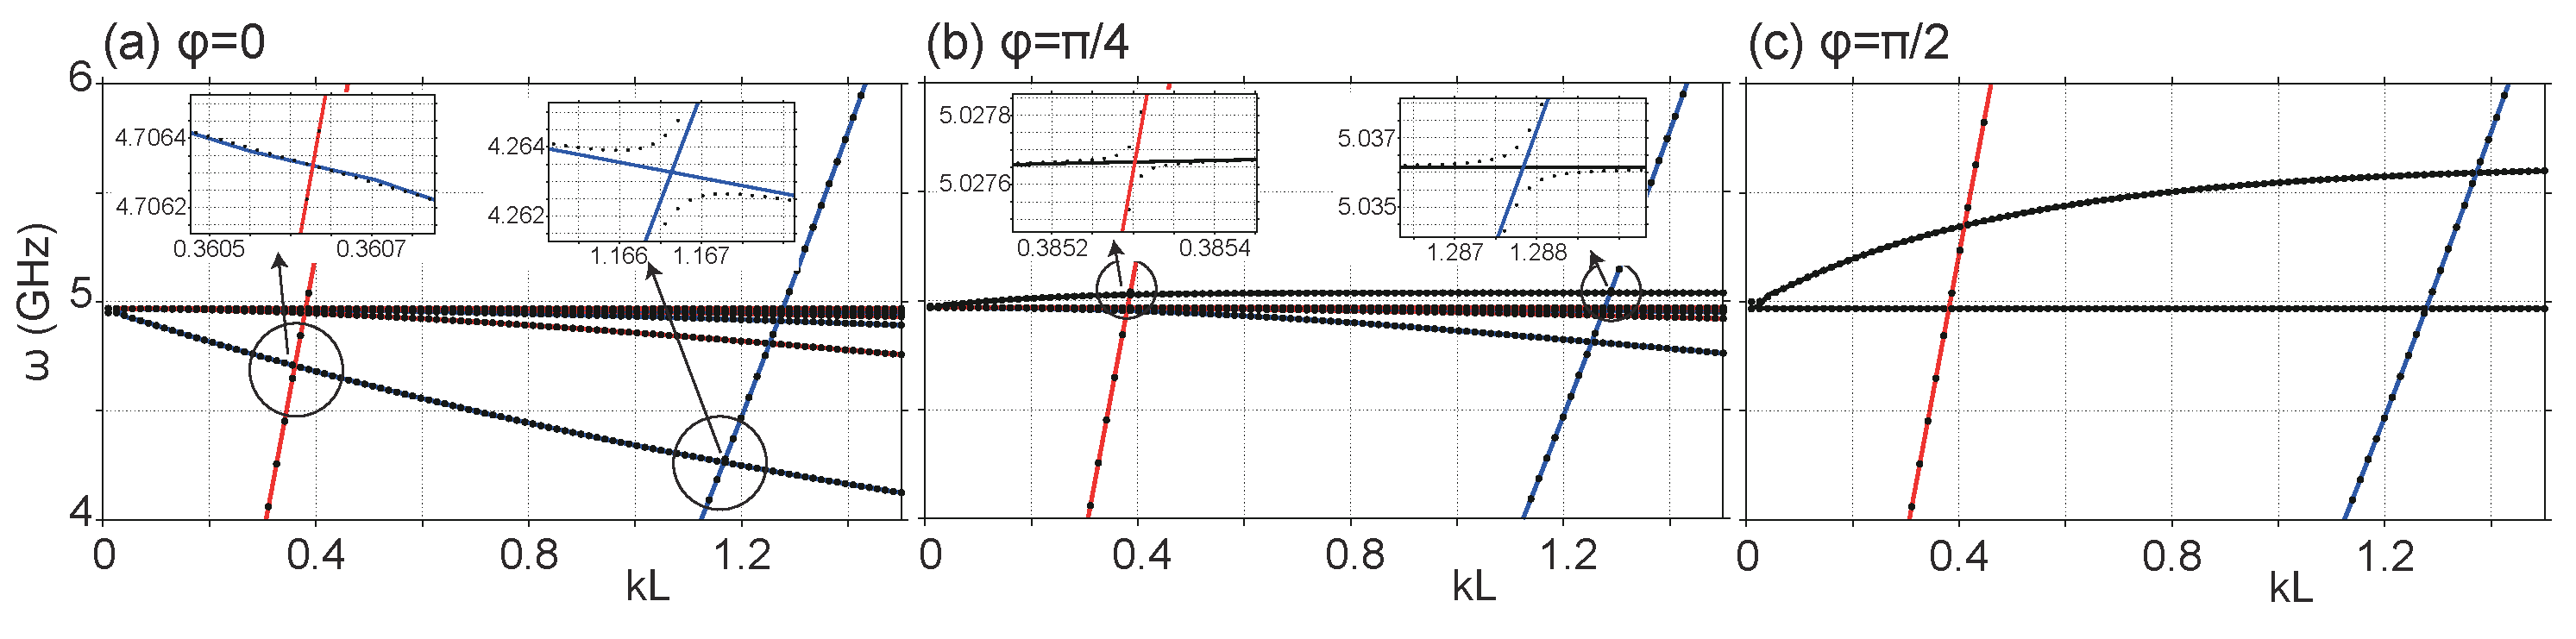
\includegraphics[width=\columnwidth]{fig/Bands.pdf}
        }
        \subfigure[After]{
            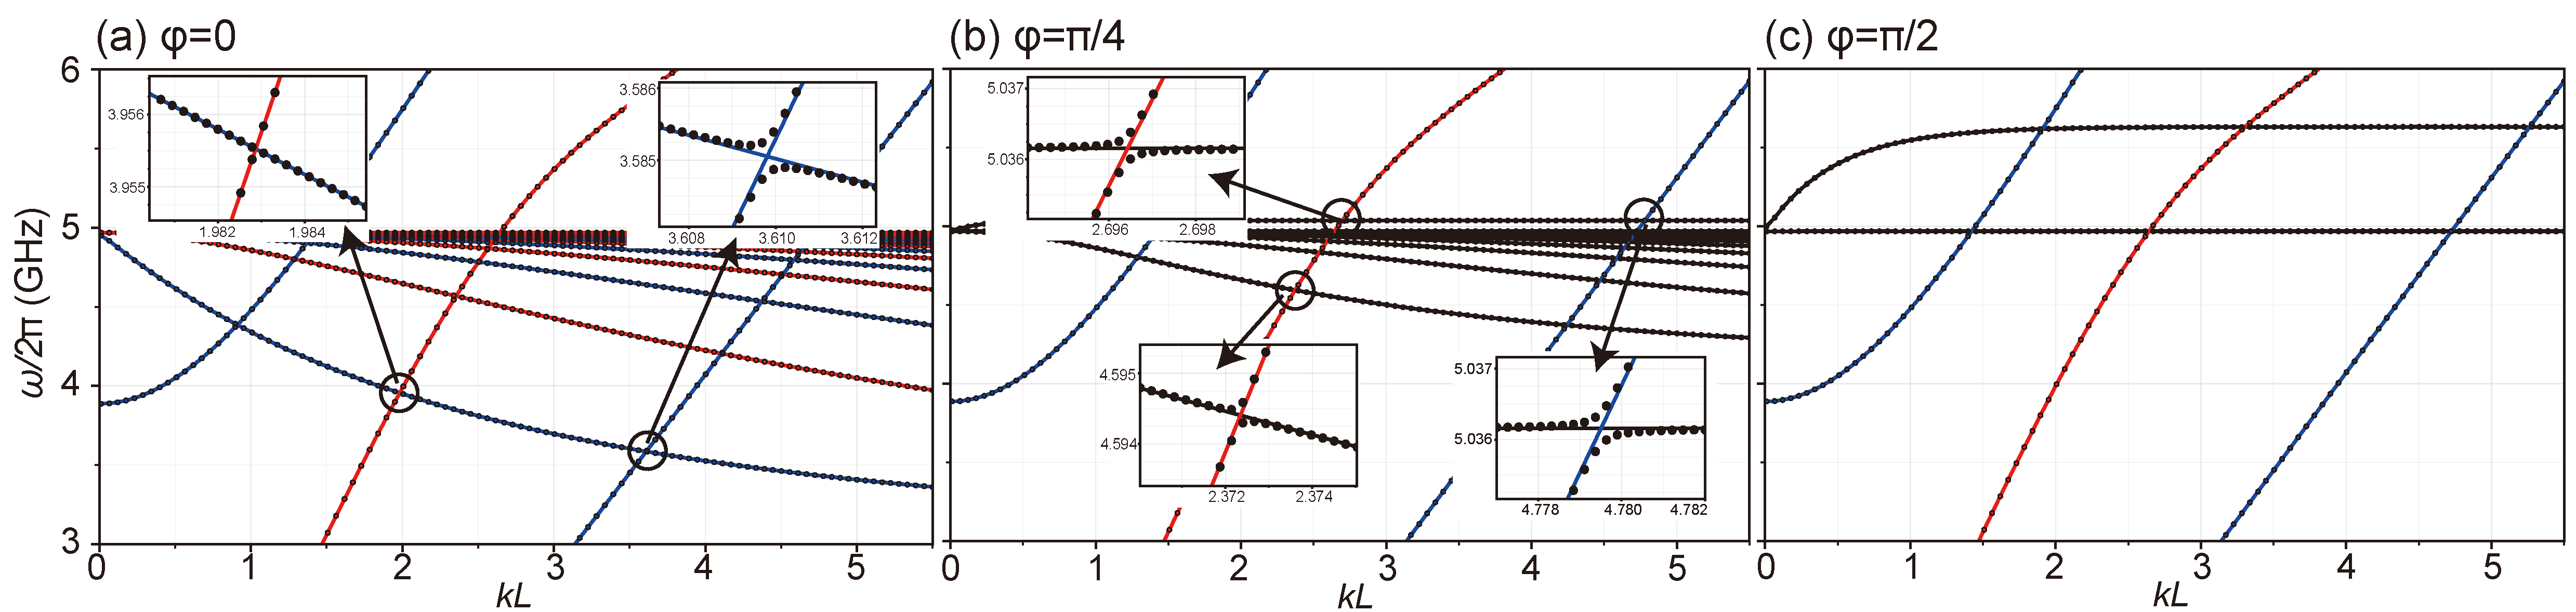
\includegraphics[width=\columnwidth]{fig/Bands2.pdf}
        }
    \end{center}
\end{figure}

\section{Changes in the main text}
\begin{enumerate}
    \item Below figure 2, $\gamma=29.8$ GHz/T $\to$ $\gamma/2\pi=29.8$ GHz/T
    \item ``... gaps of several MHz'' $\to$ ``...gaps on the order of $0.1$--$1$ MHz'' at abstract, below Fig.~2, and conclusion.
    \item ``... order of a few MHz'' $\to$ ``... order of $1$ MHz'' at two paragraphs above conclusion.
\end{enumerate}


\end{document}